\chapter{Physics Background} \label{ch:background}

%This chapter indroduces the definitions of transverse energy, ways to measure it using different detectors, and particular examples from the STAR detector.
% \section{Nuclear Matter}
% \subsection{Phase Transitions}
% \subsection{Quark-Gluon Plasma}
% \section{Relativistic Heavy Ion Collisions}
% \subsection{RHIC and LHC}
% \subsection{Beam Generation}
% \subsection{Collision Cross Sections}
% \subsection{Models of Collision Physics}
% \subsection{Detection of Collision Products}
% \subsubsection{Tracking Detectors}
% \subsubsection{Calorimeters}
% \section{Detection of QGP Signatures}
% \subsection{Bjorken Energy Density}
% \subsection{Strangeness Enhancement}
% \subsection{Jet Quenching}
% \section{Transverse Energy}
% \section{RHIC Beam Energy Scan Program}

\section{Nuclear Matter}

\subsection{Phase Transitions}
In everyday life, we observe matter existing in four distinct phases: solid, liquid, gas, and plasma. Changes in physical conditions can lead to a transition from one of these phases to another, exemplified by the commonly observed coversion of ice to water. Distinctions among the various phases can be represented in a chart called the phase diagram.

The phase diagram consists of thermodynamic observables such as temperature and density on its axes. Curves in the phase diagram represent boundries of physical conditions at which two or more phases of matter can coexist in equilibrium. Crossing a boundary represents an abrupt transition from one phase to another; this abruptness is mathematically characterized by the discontinuity in the change of the derivative of the free energy -- a thermodynamic varible -- with respect to the physical quantities in the axes. There can also be regions in the diagram representing the ranges of physical conditions in which a smooth phase transition can take place.

One of the main focuses of current experimental and theoretical nuclear physics research is the study of the phase diagram of nuclear matter at a range of temperatures and baryon chemical potentials. In experiments involving the collisions of heavy ions at high and low energies, different regions of the phase diagram can be probed by varying the collision energy \cite{PhysRevC.93.024901}. For instance, the high-baryon chemical potential regime corresponds to lower beam energies and higher temperatures correspond to higher beam energies. The results of these experiments and model calculations can be used to study the nature of transitions in the phase diagram.

A schematic representing the QCD phase diagram on the temperature (T) and quark chemical potential ($\mu$) plane is shown in Figure \ref{fig:PhaseDiagram} \cite{1742-6596-761-1-012066}. A second-order transition is predicted at low baryon chemical potentials (close to baryon-antibaryon symmetry) and high temperatures reminiscent of the early universe but within reach at modern facilities, specifically the Relativistic Heavy Ion Collider (RHIC) at the Brookhaven National Laboratory and the Large Hadron Collider (LHC) at CERN. At low temperatures and high chemical potentials, loose predictions have been made regarding the existence of exotic phases of high density matter, and programs, such as the Compressed Baryonic Matter experiment at the Facility for Antiproton and Ion Research in Germany, are being designed to study this region of the phase diagram.

\begin{figure}[h]
  \centering
  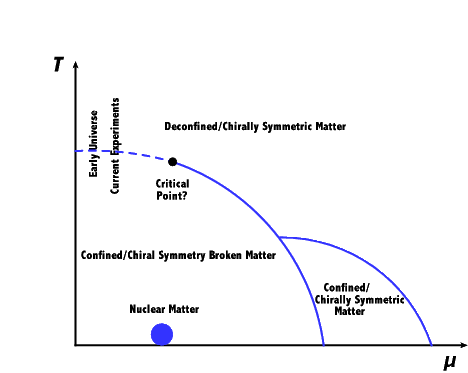
\includegraphics[width=5.5in]{figures/1742-6596-761-1-012066.png}\\
  \caption{Schematic of the QCD phase diagram \cite{1742-6596-761-1-012066}.}\label{fig:PhaseDiagram}
\end{figure}


\subsection{Quark-Gluon Plasma}
Quantum chromodynamics (QCD) -- the gauge theory of strong interaction \cite{KAPUSTA1979461, Shuryak1988} -- predicts a phase transition, at energy densities above 0.2-1 GeV/fm$^{3}$ \cite{Adam:2139456} and around a critical temperature of about 200 MeV \cite{2013arXiv1304.1452M}, of nuclear matter to a phase with quarks and gluons in thermal and chemical equilibrium representing the relevant degrees of freedom and behaving like an almost perfect quantum fluid \cite{PhysRevLett.109.152303}. This deconfined state of quarks and gluons is termed the quark-gluon plasma (QGP) in analogy to the quantum electrodynamical plasma phase of matter. The deconfinement is what the weakening of the strong interaction due to the polarization of the QCD vacuum is expected to lead to at high energies. The expectation of this phase transition also makes sense in terms of the chiral symmetry of the QCD Lagrangian, which is spontaneously broken at low temperatures, but restored at high temperatures, providing a sufficient condition for the deconfinement.
% Existence of QGP in the early universe
% Production of QGP in the lab

\section{Relativistic Heavy Ion Collisions}

% \subsection{RHIC and LHC}
% \subsection{Beam Generation}
% \subsection{Collision Cross Sections}
% \subsection{Models of Collision Physics}
% \subsection{Detection of Collision Products}
% \subsubsection{Tracking Detectors}
% \subsubsection{Calorimeters}
% \section{Detection of QGP Signatures}
% \subsection{Bjorken Energy Density}
% \subsection{Strangeness Enhancement}
% \subsection{Jet Quenching}
% \section{Transverse Energy}
% \section{RHIC Beam Energy Scan Program}
